\chapter{Background}


The desire to get more computing power and better reliability by orchestrating a number of low cost commercial off-the-shelf computers has given rise to a variety of architectures and configurations.
\\~\\
The computer clustering approach usually (but not always) connects a number of readily available computing nodes (e.g. personal computers used as servers) via a fast local area network. The activities of the computing nodes are orchestrated by "clustering middleware", a software layer that sits atop the nodes and allows the users to treat the cluster as by and large one cohesive computing unit, e.g. via a single system image concept.
\\~\\
Computer clustering relies on a centralized management approach which makes the nodes available as orchestrated shared servers. It is distinct from other approaches such as peer to peer or grid computing which also use many nodes, but with a far more distributed nature.
\\~\\
A computer cluster may be a simple two-node system which just connects two personal computers, or may be a very fast supercomputer. A basic approach to building a cluster is that of a Beowulf cluster which may be built with a few personal computers to produce a cost-effective alternative to traditional high performance computing. An early project that showed the viability of the concept was the 133 nodes Stone Soupercomputer.[4] The developers used Linux, the Parallel Virtual Machine toolkit and the Message Passing Interface library to achieve high performance at a relatively low cost.
\\~\\
Although a cluster may consist of just a few personal computers connected by a simple network, the cluster architecture may also be used to achieve very high levels of performance. The TOP500 organization's semiannual list of the 500 fastest supercomputers often includes many clusters, e.g. the world's fastest machine in 2011 was the K computer which has a distributed memory, cluster architecture.
\\~\\
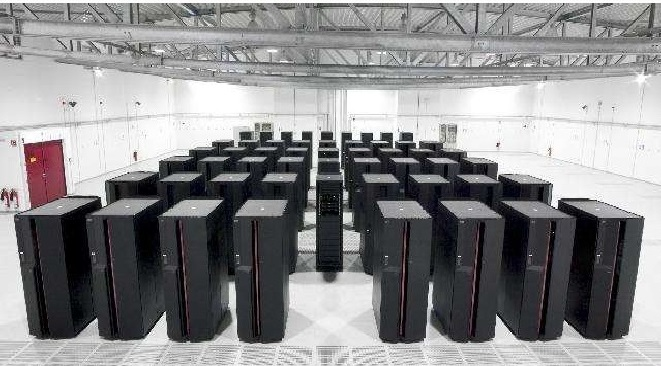
\includegraphics[width=0.75\columnwidth]{./img.jpg} % Example image

